\title{LEZIONE 2 12/03/2020}\newline
\textbf{link} \href{https://web.microsoftstream.com/video/7f38ca42-5bcf-4a08-b9cf-d42ca1289062}{clicca qui}
\section{Cinematica di un corpo}
\subsection{Definizioni}
\begin{itemize}
    \item \textbf{Corpo}: Un corpo è un insieme continuo di infiniti punti che assume dimensioni finite.
    \item \textbf{Posizione del corpo}: è l'insieme di tutti i vettori posizione relativi a ciascun punto appartenente al corpo.
    \item \textbf{Spostamento, velocità, accellerazione}: definiamo spostamento, velocità, accellerazione, come l'insieme di tutti i vettori spostamento, velocità, accellerazione relativi a ciascun punto appartenente al corpo.
    \item \textbf{Moto piano}: in questo corso faremo sempre riferimento a un moto piano, che rappresenta il caso in cui tutti i vettori posizione, velocità e accellerazione di tutti i punti appartenenti al corpo sono paralleli a un piano, detto \textbf{piano direttore}.
    \item \textbf{Spostamento infinitesimo}: lo spostamento infinitesimo è una condizione di moto per cui ogni punto che appartiene al corpo subirà uno spostamento di dimensione infinitesima.
    \item \textbf{Atto di moto}: l'atto di moto è l'insieme delle velocità di tutti i punti che appartengono al corpo nell'istante di tempo generico considerato. L'atto di moto rappresenta una "fotografia istantanea" del suo campo di velocità. Possiamo definire un'analogia fra lo spostamento infinitesimo e l'atto di moto: siccome la velocità di un generico punto $P$ è $\vec{v_P} = \frac{d \vec{P}}{dt}$, l'atto di moto può essere visto come lo spostamento infinitesimo di $P$ fratto l'intervallo di tempo infinitesimo $dt$ in cui esso avviene. Perciò tutte le regole cinematiche che definiremo per l'atto di moto varranno anche per lo spostamento infinitesimo.
\end{itemize}
Tutte le definizione appena viste valgono per un qualsiasi corpo, ma noi \textbf{nel corso vedremo solo corpi rigidi}.\newline
Per un corpo deformabile ci servono $\infty^2$ gradi di libertà (caso piano) per descrivere ciascuno degli infiniti punti che lo rappresentano.\newline
Nel caso di un corpo rigido saranno sufficienti $3$ gradi di libertà per definire la posizione del corpo nel piano.
\subsection{Corpo rigido}
Un \textbf{corpo} si definisce \textbf{rigido} se esso può definire solamente \textbf{spostamenti rigidi}. Uno \textbf{spostamento} si può definire \textbf{rigido} se a fronte di esso il corpo \textbf{non subisce alcuna variazione nè di forma nè di dimensioni}.\newline
[immagine dagli appunti del prof]
\begin{center}
    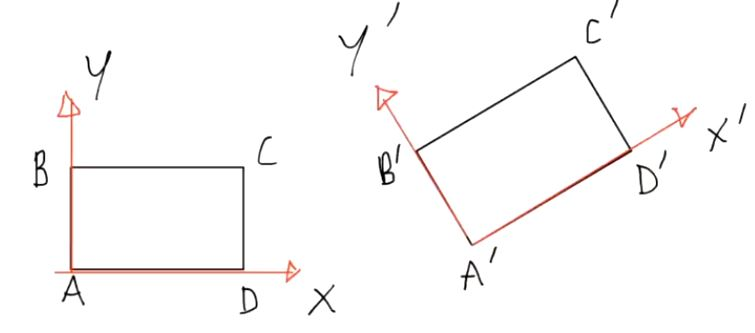
\includegraphics[height=3cm]{../lezione2/img1.JPG}
\end{center}
Più analiticamente diciamo che \textbf{uno spostamento è rigido se a seguito dello spostamento esiste un nuovo sistema di riferimento per cui la posizione del corpo rigido risulta la stessa di partenza}.\newline
Se per esempio il corpo subisce un rimpicciolimento o una deformazione a seguito dello spostamento, non siamo in presenza di uno spostamento rigido.\newline
\newline
Ne conseguono due \textbf{proprietà}:
\begin{itemize}
    \item La distanza fra due punti qualsiasi di un corpo rigido si mantiene immutata.
    \item L'angolo formato dalle rette passanti fra due coppie di punti appartenenti al corpo rimane immutato.
\end{itemize}
\ \newline
Il principale vantaggio di studiare corpi rigidi è che dobbiamo usare solo \textbf{3 coordinate} (3 gradi di libertà) per descrivere pienamente degli spostamenti.\newline
Per capire quali tre coordinate scegliere si seleziona un punto qualsiasi $A$ all'interno del corpo:
\begin{itemize}
    \item la prima è l'ascissa del punto $A$ (come per il punto), $x_A(t)$;
    \item la seconda è l'ordinata del punto $A$ (come per il punto), $y_A(t)$.
    \item La terza è la \textbf{coordinata angolare} $\phi$ di un segmento qualsiasi che collega il punto $A$ con un altro generico punto $B$ interno al corpo. Ogni punto $B$ mantiene invariata la sua distanza dal punto $A$ a seguito di un qualsiasi spostamento e, studiando come varia l'orientamento di questo segmento $AB$, sono in grado di ricostruire la posizione di ciascuno dei punti all'interno del corpo rigido. La rotazione $\phi$ avviene attorno ad un asse $z$ che esce dal piano del corpo rigido. Qualsiasi segmeno all'interno del corpo subirà la stessa variazione angolare (stessa rotazione): la rotazione $\phi$ è una proprietà dell'intero corpo rigido.
\end{itemize}
[immagine dagli appunti del prof]
\begin{center}
    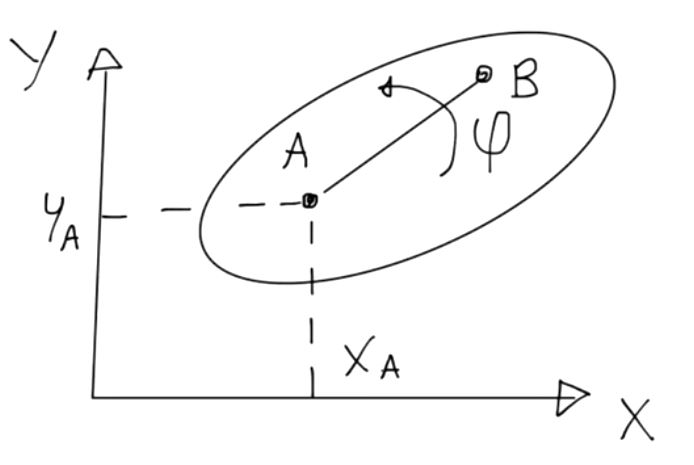
\includegraphics[height=3cm]{../lezione2/img2.JPG}
\end{center}
\subsection{Moto in grande}
\subsubsection{Traslazione} 
E' un moto nel quale un corpo non varia il proprio orientamento, ovvero in cui la coordinata angolare rimane costante. Tutti i punti del corpo subiranno lo stesso esatto spostamento, dunque $\vec{v_A} = \vec{v_B} = \dots$, $\vec{a_A} = \vec{a_B} = \dots$ e le traiettorie di ciascun punto saranno le stesse.\newline
[immagine dagli appunti del prof]
\begin{center}
    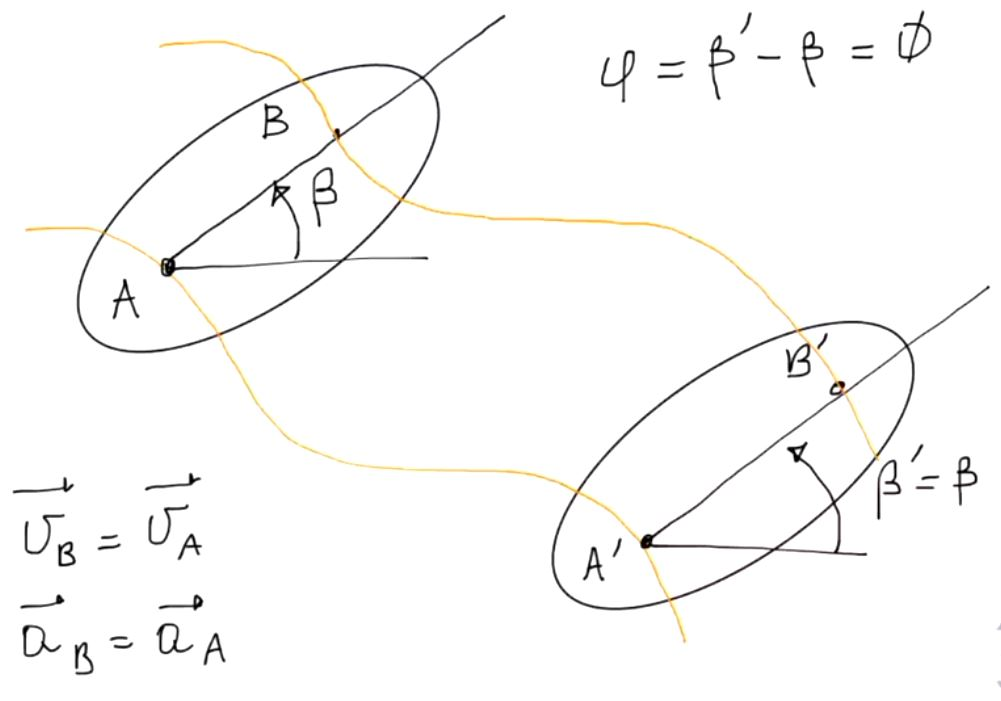
\includegraphics[height=3cm]{../lezione2/img3.JPG}
\end{center}
\subsubsection{Rotazione} 
E' un moto nel quale un punto (anche esterno al corpo), detto centro di rotazione, mantiene la sua posizione fissa durante lo spostamento. Tutti gli altri punti invece subiranno una rotazione $\phi$. La traiettoria di ogni punto seguirà un moto circolare. Possiamo definire un vettore detto $\vec{\phi} = \phi \vec{k}$ ovvero con direzione uscente dal piano.
\newline[immagine dagli appunti del prof]
\begin{center}
    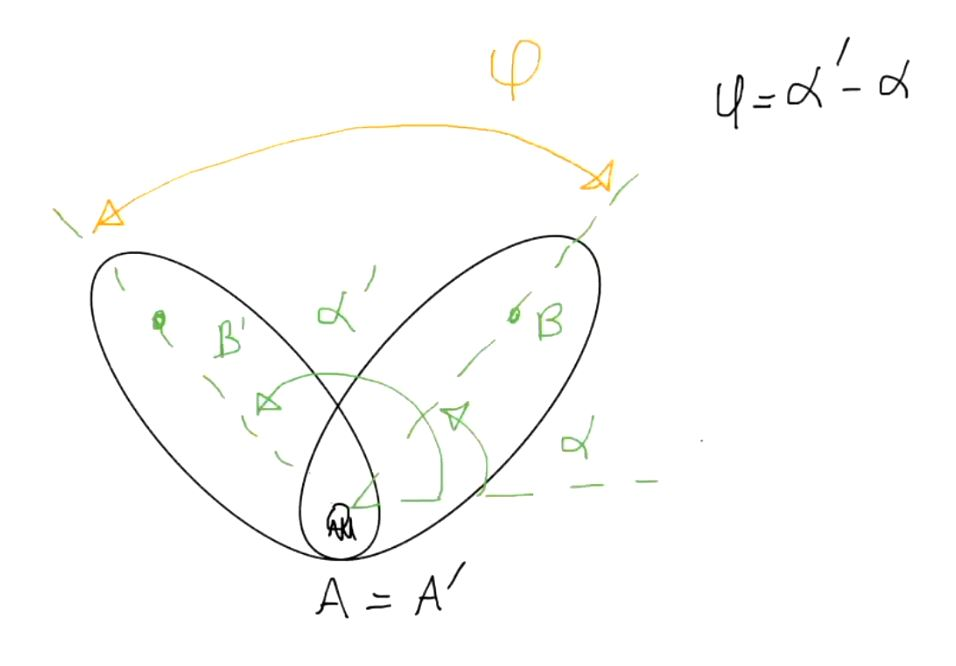
\includegraphics[height=3cm]{../lezione2/img4.JPG}
\end{center}
\subsubsection{Rototraslazione}
Il corpo rigido andrà a modificare la propria posizione senza però che sia possibile individuare un punto che rimane fermo. Per studiare il moto rototraslatorio si può lavorare considerando due spostamenti successivi, prima una traslazione e poi una rotazione.
\newline[immagine dagli appunti del prof]
\begin{center}
    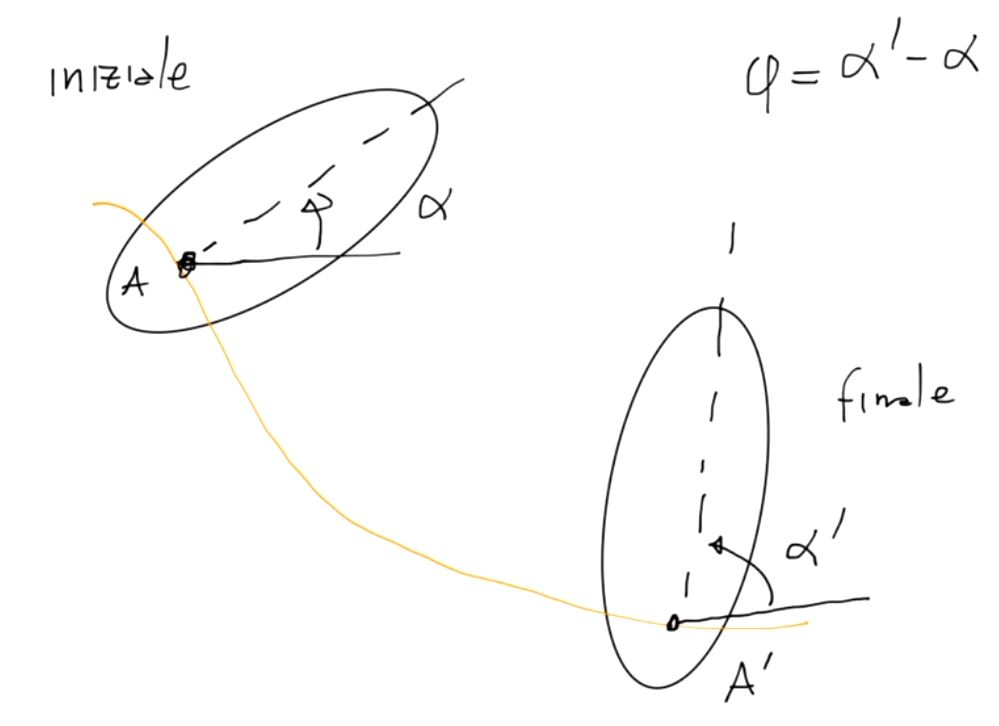
\includegraphics[height=3cm]{../lezione2/img5.JPG}
\end{center} 
\subsection{Moto in piccolo (Atto di moto)}
Per \textbf{atto di moto} si intende un moto in cui gli spostamenti e le rotazioni sono di dimensione infinitesima. \textbf{L'atto di moto rappresenta una "fotografia istantanea" del campo di velocità del corpo}.\newline
\newline
Andando ad osservare movimenti in piccolo quindi ci ritroviamo difronte a moti \textbf{o rotatori o traslatori}, non rototraslatori: se la velocità di tutti i punti è uguale in modulo direzione e verso, l'atto di moto è di tipo traslatorio; viceversa, se esiste un punto, detto \textbf{centro di istantanea rotazione}, in cui la velocità è nulla, siamo in presenza di un moto di tipo rotatorio.\newline
\newline
\textbf{es.} Esempio di rotazione:\newline
[immagine dagli appunti del prof]
\begin{center}
    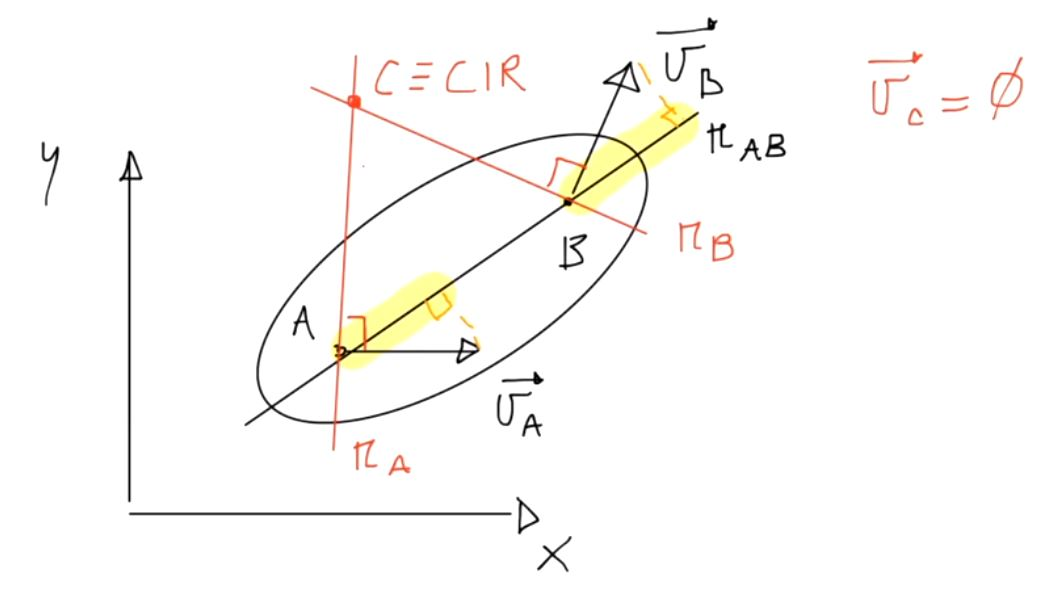
\includegraphics[height=3cm]{../lezione2/img6.JPG}
\end{center}
Presi i punti $A$ e $B$ interni al corpo e le rispettive velocità $\vec{v_A}$ e $\vec{v_B}$, essendo il corpo rigido, le proiezioni delle velocità sulla retta $r_{AB}$ devono essere di medesima lunghezza (nell'immagine: evidenziate in giallo).\newline
Consideriamo ora le rette $r_A$ passante per $A$ e perpendicolare a $\vec{v_A}$ e la retta $r_B$ passante per $B$ e perpendicolare a $\vec{v_B}$; tutti i punti che si trovano sulla retta $r_A$ devono avere velocità perpendicolare alla retta stessa (analogo per la retta $r_B$), perchè altrimenti il corpo subirebbe una deformazione, quindi tutti i punti su $r_A$ (o $r_B$) devono avere velocità perpendicolare a $\vec{v_A}$ (o $\vec{v_B}$). Il punto $C$ di intersezione di queste due rette dovrebbe avere velocità perpendicolare sia a $\vec{v_A}$ sia a $\vec{v_B}$, ma questo è possibile solo se $\vec{v_C} = 0$, dunque il punto $C$ è il centro di istantanea rotazione del corpo rigido e siamo dunque in presenza di una rotazione.\newline
\rule{\textwidth}{0,4pt}
\ \newline
\textbf{oss.} Il centro di istantanea rotazione differisce dal centro di rotazione (dei moti in grande), il primo ha velocità nulla solo nell'istante che stiamo considerando, mentre il secondo è fermo per tutto l'arco della rotazione. In poche parole il centro di istantanea rotazione ha velocità nulla, ma la sua accellarazione può non esserlo.\newline
\newline
\textbf{es.} Esempio di traslazione:\newline
[immagine dagli appunti del prof]
\begin{center}
    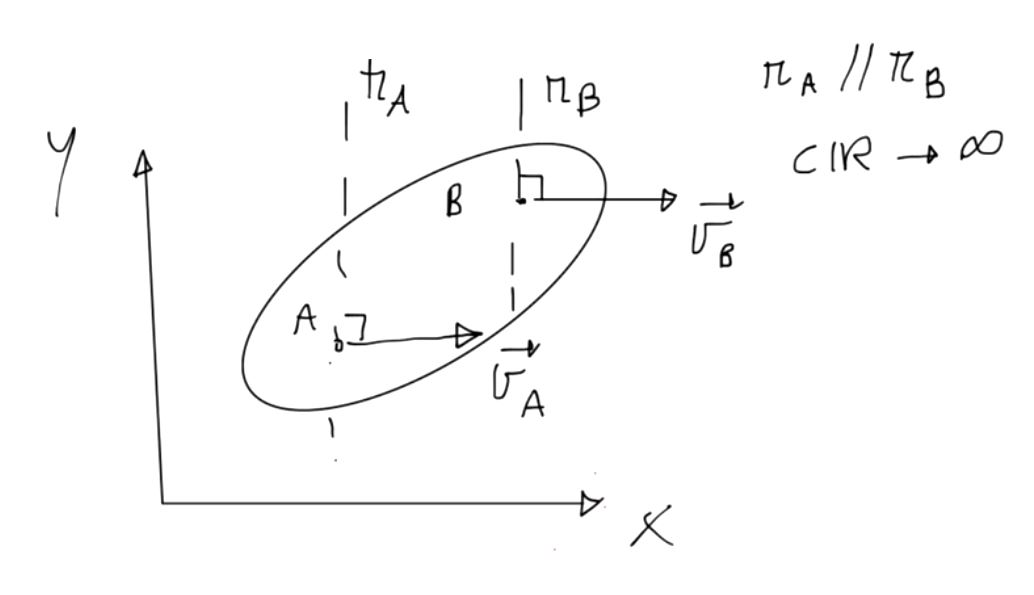
\includegraphics[height=3cm]{../lezione2/img7.JPG}
\end{center}
In questo caso le rette $r_A$ e $r_B$ sono parallele e non si incontrano mai, il centro di istantanea rotazione non è definibile e dunque il moto e traslatorio.\newline
\rule{\textwidth}{0,4pt}
\ \newline
\textbf{es.} Esempio di moto di un corpo non rigido:\newline
[immagine dagli appunti del prof]
\begin{center}
    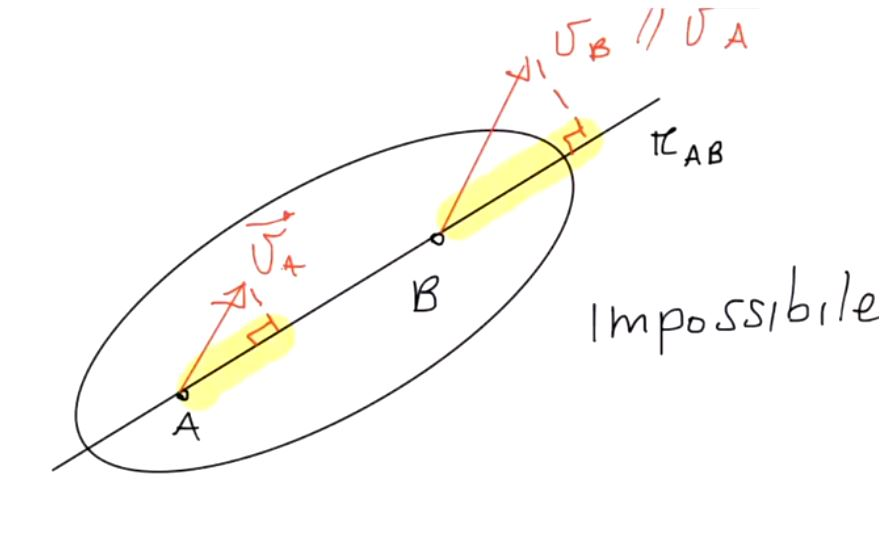
\includegraphics[height=3cm]{../lezione2/img8.JPG}
\end{center}
Se i due punti $A$ e $B$ hanno $\vec{v_A}$ e $\vec{v_B}$ di modulo diverso, le proiezioni (in giallo) di queste due velocità sulla retta $r_{AB}$ non sono identiche e dunque il corpo si sta deformando. In tutti i casi in cui le proiezioni delle velocità sulla retta sono diverse sicuramente rappresentano deformazioni del corpo, e quindi moti non rigidi.\newline
\rule{\textwidth}{0,4pt}
\ \newline
\textbf{es.} Un altro esempio di rotazione:\newline
[immagine dagli appunti del prof]
\begin{center}
    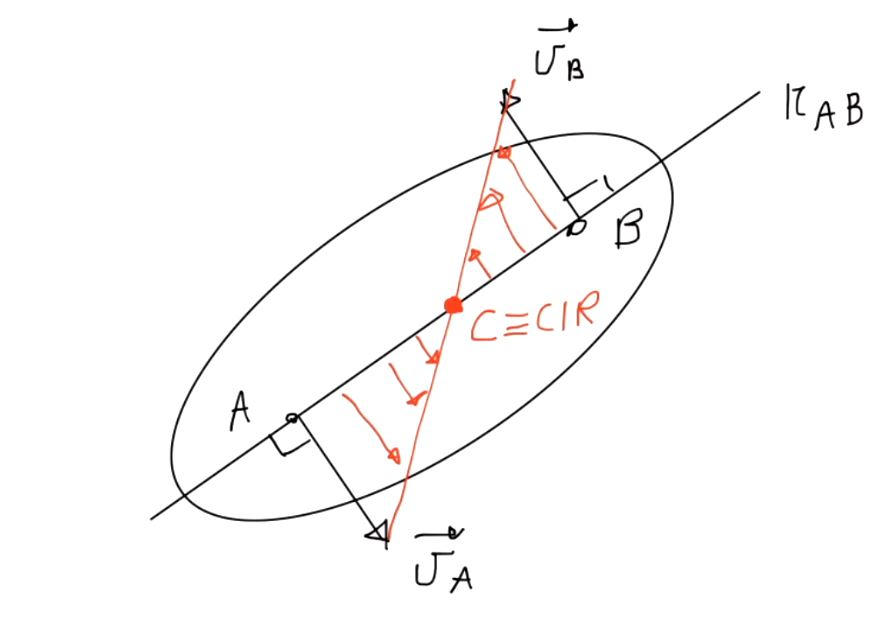
\includegraphics[height=3cm]{../lezione2/img9.JPG}
\end{center}
Se i due punti $A$ e $B$ hanno $\vec{v_A}$ e $\vec{v_B}$ di direzione opposta, la congiungete fra le due velocità (disegnata in rosso) ci mostra che la velocità di tutti i punti lungo il segmeno $AB$ deve diminuire man mano che ci avviciniamo al punto $C$, che quindi ha velocità nulla e rappresenta il centro di istantanea rotazione.\newline
\rule{\textwidth}{0,4pt}
\ \newline
\textbf{es.} Un altro esempio di rotazione:\newline
[immagine dagli appunti del prof]
\begin{center}
    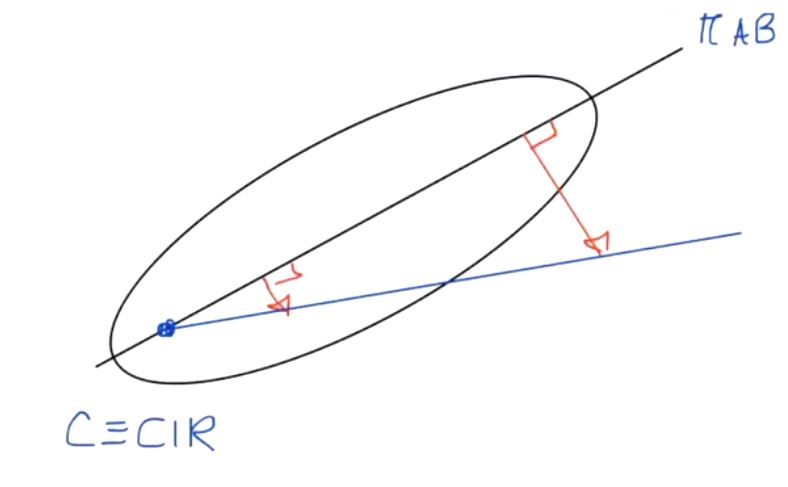
\includegraphics[height=3cm]{../lezione2/img10.JPG}
\end{center} 
Se i due punti $A$ e $B$ hanno $\vec{v_A}$ e $\vec{v_B}$ direzione e verso uguali (sono parallele) ma modulo diverso, ancora una volta, la congiungete fra le due velocità (disegnata in rosso) ci mostra che la velocità di tutti i punti lungo il segmeno $AB$ deve diminuire man mano che ci avviciniamo al punto $C$, che quindi ha velocità nulla e rappresenta il centro di istantanea rotazione.\newline
\rule{\textwidth}{0,4pt}
\subsection{Cinematica del corpo rigido}
[immagine dagli appunti del prof]
\begin{center}
    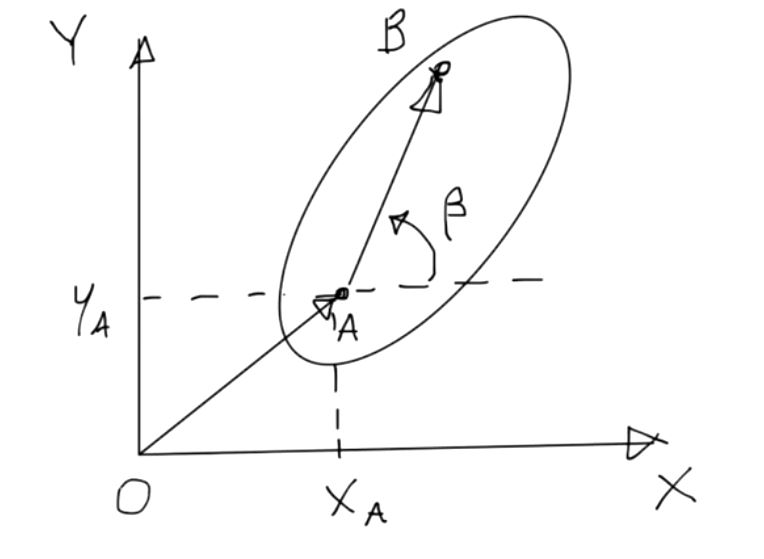
\includegraphics[height=3cm]{../lezione2/img11.JPG}
\end{center}
Sia in un piano un corpo rigido, siano due punti qualsiasi $A$ e $B$ appartenenti a questo e sia $\beta$ l'angolo fra il segmento $AB$ e l'asse orizzontale delle ascisse.\newline
\newline
Ci servono \textbf{tre coordinate idipendenti} (tre gradi di libertà) per definire l'evoluzione temporale della traslazione di un punto generico del punto $A = (x_A(t), y_A(t), \beta(t))$. Se queste tre coordiante indipendenti sono note, allora si può studiare l'evoluzione temporale anche dell'intero corpo rigido.\newline
\newline
Supposte note queste tre coordiante $x_A(t), y_A(t), \beta(t)$, vogliamo definire velocità, posizione e accellerazione del corpo.\newline
\newline
Da notare è che, se invece di $B$ prendessimo un altro generico punto $P$ appartenente al corpo, l'angolo $\alpha$ formato fra il segmento $AP$ e l'asse orizzontale delle ascisse differisce dall'angolo $\beta$ a meno di una costante $\gamma$ a fronte di qualsiasi spostamento.
\subsubsection{Posizone}
Per definire la posizione di un punto generico di un corpo, per esempio il punto $B$, posso scrivere una realazione vettoriale che lega tre vettori:
\begin{itemize}
    \item il vettore $AO$;
    \item il vettore $AB$;
    \item il vettore $OB$.
\end{itemize}
Questi tre vettori sono legati dall'equazione: $(B-O) = (A-O) + (B-A)$. Il vettore $A-O$ è dato da $x_A \vec{i} + y_A \vec{j}$; il vettore $B-A$ è dato dal vettore $AB$ (dal suo modulo) moltiplicato per $e^{i \beta}$, quindi $AB \cdot e^{i \beta}$. Essendo tutti questi termini noti posso definire la generica posizione del punto $B$.
\subsubsection{Velocità}
La velocità del punto $B$ è $\vec{v_B} = \frac{d}{dt}(B-O) = \frac{d}{dt}(A-O) + \frac{d}{dt}(B-A)$. Dunque andiamo ad eseguire queste derivate: $\vec{v_B} = \vec{v_A} + \frac{d}{dt} (AB \cdot e^{i \beta})$, dove il primo termine è la semplice velocità del punto $A$, il secondo membro è la derivata di ciò che abbiamo detto anche al punto precedente. Dunque $\vec{v_B} = \vec{v_A} + i \dot{\beta} \cdot AB \cdot e^{i \beta} = \vec{v_A} + \dot{\beta} \cdot AB \cdot e^{i(\beta + pi/2)}$. Da notare è che $\dot{\beta} = \frac{d \beta}{d t}$ e che, siccome avevamo visto che per un qualunque altro punto ($P$) si ha un angolo ($\alpha$) che differisce da $\beta$ per una costante ($\gamma$), quindi, $\dot{\beta} = \dot{\alpha} = \dots = \omega$, che rappresenta la \textbf{velocità angolare} del corpo rigido. Possiamo anche definire un vettore velocità angolare $\vec{\omega} = \omega \vec{k} = \dot{\beta} \vec{k}$.\newline
\newline
A partire dal vettore $\vec{\omega}$ possiamo definire il senso di rotazione del corpo rigido con la regola della mano destra (ponendo il pollice nella direzione del vettore, otteniamo la rotazione nel senso delle dita che si avvolgono).\newline
\newline
Tutti i punti del corpo ruotano con la stessa velocità angolare.\newline
La velocità del punto $B$, $\vec{v_B} = \vec{v_A} + \omega \cdot AB \cdot e^{i(\beta + \pi/2)}$, può essere vista come somma di due componenti:
\begin{itemize}
    \item $\vec{v_A}$: la velocità con cui trasla il punto $A$.
    \item $\omega \cdot AB \cdot e^{i(\beta + \pi/2)}$: velocità di un punto che si muove di moto rotatorio, in particolare è la velocità con cui si muove il punto $B$ di moto circolare attorno al punto $A$. Questa componente è anche detta $\vec{v}_{BA}$, ovvero la velocità di $B$ rispetto al punto $A$.
\end{itemize}
\ \newline
Riassumendo: \newline
\textbf{teor.} \textbf{Teorema di Rivals per le velocità}
\[
    \vec{v_B} = \vec{v_A} + \omega \cdot AB \cdot e^{i(\beta + \pi/2)} = \vec{v_A} + \vec{v_{BA}}
\]
oppure in forma abbreviata
\[
    \vec{v_B} = \vec{v_A} + \vec{\omega}\land(B-A)
\]
dove $\land$ rappresenta un prodotto vettoriale.
\subsubsection{Accellerazione}
Partendo dalla formula $\vec{v_B} = \vec{v_A} + \dot{\beta} \cdot AB \cdot e^{i(\beta + \pi/2)}$, l'accellerazione si ottiene derivando queste due componenti rispetto al tempo.\newline
Quindi
\[
    \vec{a_B} = \vec{a_A} + \ddot{\beta} \cdot AB \cdot e^{i(\beta+\pi/2)}-AB \cdot \dot{\beta}^2 e^{i \beta}
\]
Il \textbf{primo termine è l'accellerazione del punto $A$}. Il \textbf{secondo e terzo termine} rappresentano l'\textbf{accellerazione tangenziale} $\vec{a_{BA}}^{(t)}$ e \textbf{normale} $\vec{a_{BA}}^{(n)}$ \textbf{del punto $B$} mentre si muove di moto circolare \textbf{attorno al punto $A$}, che sommati rappresentano $\vec{a_{BA}}$. In questo moto ciroclare il $B$ ha velocità angolare $\omega = \dot{\beta}$ e accellerazione angolare $\dot{\omega} = \ddot{\beta}$. Possiamo anche qui andare a definire il vettore $\vec{\dot{\omega}} = \ddot{\beta}\vec{k}$.\newline
\newline
Partendo invece da $\vec{v_B} = \vec{v_A} + \vec{\omega}\land(B-A)$ e derivando otteniamo $\vec{a_B} = \vec{a_A} + \dot{\vec{\omega}}\land (B-A) + \vec{\omega} \land \frac{d}{dt}(B-A)$, dove $\frac{d}{dt}(B-A)$ è esattamente la quantità scritta prima. Possiamo quindi scrivere l'accelerazione come 
\[
    \vec{a_B}= \vec{a_A} + \dot{\vec{\omega}} \land (B-A) + \vec{\omega} \land \vec{\omega} \land (B-A)
\]
dove il secondo e terzo termine rappresentano l'accellerazione tangenziale $\vec{a_{BA}}^{(t)}$ e normale $\vec{a_{BA}}^{(n)}$ del punto $B$ mentre si muove di moto circolare attorno al punto $A$.\newline
\newline
\textbf{teor.} \textbf{Teorema di Rivals per le accellerazioni}
\[
    \vec{a_B}= \vec{a_A} + \dot{\vec{\omega}} \land (B-A) + \vec{\omega} \land [\vec{\omega} \land (B-A)]
\]